\documentclass[tikz, border=5pt]{standalone} % Use standalone for PNG/SVG export
\usepackage{tikz}
\usepackage{tikz-network}
\usepackage{amsmath}
\usepackage{amsfonts}
\usepackage{amssymb}
\usetikzlibrary{positioning, backgrounds}

\begin{document}
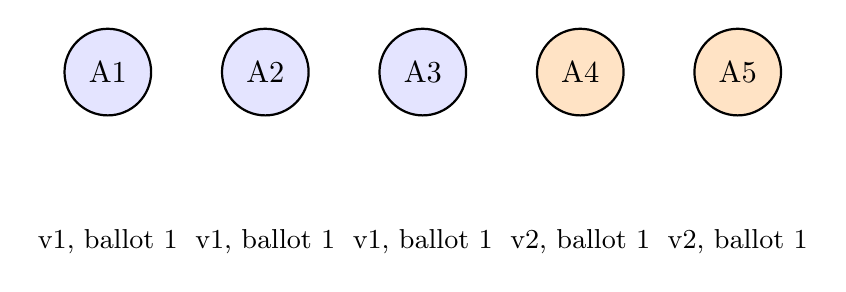
\begin{tikzpicture}[node distance=2.5cm, every node/.style={scale=1.1}]
    % Draw acceptor circles
    \foreach \i in {1,...,5} {
        \node[circle, draw, thick, minimum size=1cm] (A\i) at (\i*2,0) {A\i};
    }

    % Accepted value indications
    % A1, A2, A3 accepted v1 in ballot 1
    \node[below=1.3cm of A1] (lA1) {{\small v1, ballot 1}};
    \node[below=1.3cm of A2] (lA2) {{\small v1, ballot 1}};
    \node[below=1.3cm of A3] (lA3) {{\small v1, ballot 1}};

    % A4, A5 accepted v2 in ballot 1
    \node[below=1.3cm of A4] (lA4) {{\small v2, ballot 1}};
    \node[below=1.3cm of A5] (lA5) {{\small v2, ballot 1}};

    % Optional: Highlight with color
    \begin{scope}[on background layer]
        % Fill v1 acceptors (A1, A2, A3) with light blue
        \foreach \i in {1,2,3} {
            \fill[blue!15, opacity=0.7] (A\i) circle [radius=0.55];
        }
        % Fill v2 acceptors (A4, A5) with light orange
        \foreach \i in {4,5} {
            \fill[orange!30, opacity=0.75] (A\i) circle [radius=0.55];
        }
    \end{scope}

    % Title
    % \node[above=1.2cm of A3] {\textbf{Fast Paxos: Acceptor States in Ballot 1}};
\end{tikzpicture}
\end{document}